\documentclass{article}
\usepackage{graphicx}
\usepackage[margin=1.5cm]{geometry}
\usepackage{amsmath}

\begin{document}

\title{Lab Activity: Smashing Things Together (Momentum)}
\author{Prof. Jordan C. Hanson}

\maketitle

\section{Introduction}
This lab activity demonstrates momentum conservation through the use of carts that repel each other via magnets, and also simply collide.  Figure \ref{fig:carts} demonstrates the general setup. When momentum is conserved between two objects labeled 1 and 2, with $i$ and $f$ referring to the initial and final states,
\begin{equation}
p_{1i} + p_{2i} = p_{1f} + p_{2f}
\end{equation}

\begin{figure}[ht]
\centering
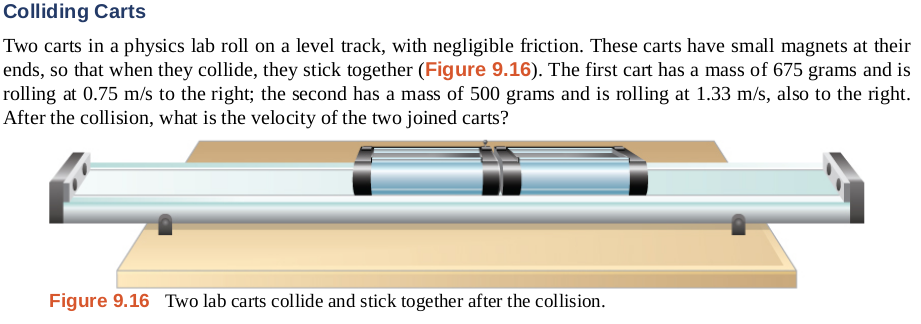
\includegraphics[width=0.6\textwidth,trim=0cm 1.2cm 0cm 5cm,clip=true]{figures/carts.png}
\caption{\label{fig:carts} Carts that collide with different interaction properties.}
\end{figure}

\section{System Setup}

Set the long frictionless rail along your lab table, and ensure that it is level by adjusting the four screws at the corners.  The lab carts should not roll one way or the other if placed on the rail once it is level.  Place a motion detector at one end of the rail, and prepare a stopwatch (Google or smartphone) and ruler to measure time and distance for a stationary cart placed in the middle of the rail.  Place one cart in the middle and leave it stationary.  Place another cart near the motion detector.

\section{Measuring Momentum Conservation}

Roll the cart near the motion detector towards the stationary one at \textbf{low speed}.  (a) Use the motion detector to measure the velocity of the first cart, and the ruler and stopwatch to measure the velocity of the second.  (b) Now alter the mass of the stationary cart by added a weight to it, and repeat the experiment.  \\ \vspace{1.5cm}

The mass of the carts is 510 grams.  Do your observations match momentum conservation?  There are two cases: equal masses and unequal masses.  Record the initial and final total momentum for the first and second cases below.  Was kinetic energy conserved in either interaction?

\end{document}